%This is a template file for use of iopjournal.cls

\documentclass{iopjournal}

\usepackage{longtable}
\usepackage{booktabs}
\usepackage{amsmath}
\usepackage{amssymb}
\usepackage{hyperref}
\usepackage{xcolor}
\definecolor{revblue}{RGB}{0,51,153}

% Options
% 	[anonymous]	Provides output without author names, affiliations or
%               acknowledgments to facilitate double-anonymous peer-review

\begin{document}

\articletype{Paper}

\title{Radiomics-Integrated Multimodal 2.5D Vision Transformer Ensemble for
Lung Cancer Identification from CT Images}

\author{Limna P Das$^1$\orcid{0000-0000-0000-0000},
        Jayaraj P B$^{1,*}$\orcid{0000-0000-0000-0000},
        Joseph Johnson$^2$\orcid{0000-0000-0000-0000} and
        Seenia Fransis$^3$\orcid{0000-0000-0000-0000}}

\affil{$^1$Department of Computer Science and Engineering,
       National Institute of Technology Calicut, Kerala, India}

\affil{$^2$Department of Computer Science and Engineering,
       College of Engineering Trivandrum, Kerala, India}

\affil{$^3$Department of Artificial Intelligence and Data Science,
       Jyothi Engineering College, Kerala, India}

\affil{$^*$Author to whom any correspondence should be addressed.}

\email{jayarajpb@nitc.ac.in}

\keywords{lung cancer; radiomics; vision transformer; multimodal ensemble;
          LIDC-IDRI; XGBoost; LightGBM}

\begin{abstract}
Lung cancer is one of the main causes of cancer-related deaths globally.
Timely and accurate diagnosis of lung cancer is essential, as tumor
heterogeneity, drug resistance, and delayed detection continue to limit the
effectiveness of even advanced treatments, highlighting the need for early
detection and intelligent decision-support systems. We propose a novel
{\color{revblue}Radiomics-Integrated Multimodal Vision Transformer Ensemble (RIM-Former)}
fusing hand-crafted radiomic features (PyRadiomics) with deep semantic
embeddings from a pre-trained medical Vision Transformer RAD-DINO in a 2.5D
multi-slice paradigm. The proposed model effectively combines these
complementary feature sets to leverage the benefits of both radiomics and deep
learning approaches. {\color{revblue}For each 3D lung nodule volume, five composite images at
anchor depths of 16, 24, 32, 40, and 48 are processed by the frozen Vision
Transformer, averaging their 768-dimensional class tokens into a global
representation. This vector is concatenated with 1,218 radiomic features to
form a 1,986-dimensional fused representation, which is fed into an ensemble of
XGBoost and LightGBM classifiers trained via patient-level Stratified 5-Fold
Cross-Validation.} Evaluated on the publicly accessible LIDC-IDRI benchmark
($N=1{,}393$ nodules from 1,018 CT scans), our model achieves an AUC of
0.9902, an Accuracy of 97.11\%, a Sensitivity of 90.28\%, and a Specificity of
99.37\%. {\color{revblue}External validation on the LNDb dataset yields an AUC of 0.8971 and a
Precision of 97.41\%, demonstrating robust cross-scanner generalizability.}
Critically, unlike prior methods that delete ambiguous Score~3 nodules or
perform slice-level splitting, our pipeline retains all indeterminate nodules
and prevents data leakage. These findings demonstrate that this strategy may
improve diagnostic accuracy and support the development of personalized
treatment plans for lung cancer management. The code and data underlying this
study's conclusions are publicly accessible at
\url{https://github.com/josephjohnson10/Radiomics.git}.
\end{abstract}

\section{Introduction}\label{sec1}

Lung cancer is a malignant disease caused by abnormal cells in the lungs that
proliferate out of control. It is a serious public health issue due to its high
morbidity and mortality rate. With the greatest mortality rates among both men
and women, lung cancer is the second most frequent cancer globally and the
primary cause of cancer-related deaths. Lung cancer is the most deadly type of
cancer, with an anticipated 2.21 million cases recorded and 1.80 million deaths
in 2020, according to the World Health Organization (WHO). Tobacco usage and
cigarette smoking account for about 90\% of cases of lung cancer. However,
other contributing factors include radon gas exposure, asbestos, air pollution,
and chronic pulmonary infections, which can also lead to lung carcinogenesis.

Lung cancer is broadly classified into two histological categories, which
differ in their growth rate and metastatic behavior: Small-Cell Lung Carcinoma
(SCLC) and Non-Small Cell Lung Carcinoma (NSCLC). NSCLC includes
adenocarcinoma (gland-forming), squamous cell carcinoma, and large-cell
carcinoma histological subtypes, and represents approximately 85\% of all new
lung cancer cases. SCLC accounts for the remaining 15\%.

Radiomics is the process of extracting quantitative, image-based features from
standard-of-care medical images and subsequently analyzing these features using
conventional biostatistical or Artificial Intelligence (AI) methods. The
concept of radiomics was first proposed in 2012 \cite{lambin2012radiomics} by
Lambin et al. Most radiomics applications are found in oncology and radiology,
including prediction of clinical outcomes, prognostication, prediction of
distant metastasis risk, assessment of cancer genetics, and prediction of
physiological events. The radiomics workflow is generally divided into four key
stages \cite{zhang2023radiomics}: \textbf{Image Acquisition} -- High-quality,
standardized imaging is obtained for diagnostic or treatment-planning purposes.
\textbf{Image Segmentation} -- Regions of Interest (ROI) are segmented using
manual, semi-automated, or fully automated approaches. Manual segmentation,
although accurate when performed by an experienced radiologist, is
labor-intensive. Semi-automated and automated methods are faster and more
reproducible \cite{lambin2012radiomics}. \textbf{Feature Extraction} --
Quantitative features are extracted from the segmented tumour region. These may
include descriptors of intensity distribution, spatial relationships between
intensity levels, texture heterogeneity patterns, shape descriptors, and
tumour--tissue interface characteristics. \textbf{Analysis} -- The most
informative features are selected based on independence from other traits,
reproducibility, and clinical relevance. These features are then analysed to
determine correlations with treatment outcomes or genetic expression.

First-order, second-order, and higher-order features are the general categories
into which radiomic features fall. First-order features describe tumor shape,
size, and voxel intensity distributions without spatial relationships.
Second-order features, sometimes referred to as texture features, capture
intratumoral heterogeneity and quantify spatial relationships between voxel
intensities. Higher-order features are extracted using mathematical filters and
transformations such as wavelet transforms, fractal analysis, and Laplacian of
Gaussian filters.

Recent studies have explored how integrating radiomics with artificial
intelligence enables novel and advanced approaches for lung cancer
prediction.

Robert et al.\ provide an in-depth exploration of radiomics, a process that
involves extracting quantitative features from medical images, such as CT, MRI,
or PET scans, and using these data to develop models for decision
support \cite{gillies2016radiomics}. The study demonstrates a paradigm change
in medical imaging that transforms images into quantitative data that can be
mined for analysis. With special reference to cancer treatment, the authors
highlight how radiomics can help with diagnosis, prognosis, and outcome
prediction. Furthermore, the paper discusses key challenges in radiomics
research, including data sharing limitations and the need for standardized
methodologies.

Sherly Angel et al.\ discuss the use of radiomics features extracted from CT
images of lung cancer patients to analyze tumor
characteristics \cite{nishanimath2021radiomics}. The study involves extracting
over 100 features from the images, performing data pre-processing and
exploratory data analysis. Exploratory data analysis revealed maximum positive
correlations between certain attributes and indicated a lack of outliers.

Junhua Chen et al.\ constructed a lung cancer diagnosis model employing
radiomics features from lung nodule images and multiple instance learning (MIL)
with deep attention \cite{chen2022lung}. With class imbalance adjustment,
attention-based MIL achieved a mean recall of 0.870, accuracy of 0.807, PPV of
0.928, NPV of 0.591, and AUC of 0.842.

B. He et al.\ designed a predictive model utilizing radiomics analysis to
determine the likelihood of a Micropapillary/Solid (MP/S) component in lung
adenocarcinoma \cite{he2021machine}. Using the PyRadiomics library, 90
radiomics features were extracted from CT images of 268 patients. Four
prediction models -- GLM, Naive Bayes, SVM, and Random Forest -- demonstrated
similar performance.

Hosseini et al.\ studied the influence of various image segmentation methods
on PET radiomics characteristics in lung cancer \cite{hosseini2021pet}. A total
of 741 radiomics features were extracted from each segmentation. The first-order
features showed top performance, while wavelet-based LLL set features achieved
the highest robustness.

Nidhi et al.\ recommended a lung cancer detection method using median filtering
for image preprocessing and mathematical morphological lung
segmentation \cite{nadkarni2019detection}. The final phase uses the SVM
classifier to determine CT scan normality.

Gautam et al.\ devised an Ensemble CNN model that precisely predicts the
severity of lung cancer nodules \cite{gautam2024lung}. The proposed method
achieved recall of 98.07\%, AUC of 94.68\%, precision of 98.58\%, F1-score of
98.33\%, and accuracy of 97.23\% on the LIDC-IDRI dataset.

Xia et al.\ developed CT image-based AI schemes to classify non-IA and IA
nodules using deep learning and radiomics features \cite{xia2020comparison}.
Compared to individual DL and radiomics schemes (AUC: $0.83\pm0.05$,
$0.87\pm0.04$), the fusion scheme significantly improves classification
performance (AUC: $0.90\pm0.03$).

Zhou et al.\ recommended a multi-head attentional feature fusion (MHA-FF)
model to distinguish IA from Pre-IA and IA subtypes \cite{zhou2023adaptive}.
Radiomics and deep CT features were combined to predict nodule subtypes,
achieving 86.83\% accuracy and 90.56\% AUC.

Ling Ma et al.\ proposed integrating radiomics and GCN features into multiple
Deep CNNs for classifying benign-malignant lung
nodules \cite{ma2023novel}. The RGD model achieved accuracy of 93.25\%,
sensitivity of 89.22\%, specificity of 95.82\%, precision of 92.46\%, F1 score
of 0.9114, and AUC of 0.9629.

The proposed work aims to improve lung cancer detection through a sequence of
well-defined steps. First, CT images are collected in DICOM format and
preprocessed using intensity normalization, noise reduction, and spatial
standardization. Radiomic characteristics are retrieved from annotated regions.
The same lung nodules are simultaneously utilized to extract deep features using
a pre-trained Vision Transformer backbone. A more thorough and instructive
representation is produced by combining these deep learning features with the
radiomic features. Machine learning ensemble models are trained using this fused
feature set. Data augmentation and oversampling strategies are used to alleviate
class imbalance. The proposed fusion model outperforms models based on separate
feature sets when assessed using standard metrics including accuracy, precision,
sensitivity, and F1-score.

%%----------------------------------------------------------------------
\section{Materials and Methods}\label{sec2}
%%----------------------------------------------------------------------

\subsection{Dataset}

The Lung Image Database Consortium and Image Database Resource Initiative
(LIDC-IDRI) is a publicly accessible medical imaging reference developed in
partnership with the National Cancer Institute (NCI), the Foundation for the
National Institutes of Health (FNIH), and the FDA \cite{armato2011lung}. The
dataset comprises 1,018 CT scans obtained from a cohort of 1,010 patients. Each
CT scan was independently reviewed and annotated by a panel of four experienced
thoracic radiologists, who identified and delineated all pulmonary nodules with
a maximum diameter exceeding 3\,mm.

Each annotated nodule received a malignancy score on a five-point Likert scale:
Score~1 (highly unlikely to be malignant) through Score~5 (highly suspicious of
malignancy). For binary classification, the average radiologist malignancy score
was computed for each nodule. Nodules with an average score greater than 3.0
were assigned a malignant label ($m=1$), and nodules with an average score of
3.0 or below were assigned a benign label ($m=0$). Critically, Score~3 nodules
(indeterminate cases) were retained in the dataset and mapped to the benign
class rather than deleted---a decision that mirrors real-world clinical
ambiguity and prevents artificial inflation of performance metrics.

Following preprocessing, a total of \textbf{1,393 pulmonary nodules} were
successfully extracted and validated: 346 malignant and 1,047 benign. The
distribution of malignancy across the base dataset is summarized in
Table~\ref{tab:dataset}.

\begin{table}[h]
\centering
\caption{Distribution of malignancy labels in the LIDC-IDRI base
dataset.}\label{tab:dataset}
\begin{tabular}{lccc}
\toprule
\textbf{Dataset} & \textbf{Malignant} & \textbf{Benign} & \textbf{Total} \\
\midrule
Base Dataset & 346 & 1,047 & 1,393 \\
\bottomrule
\end{tabular}
\end{table}

\begin{figure}[h!]
\centering
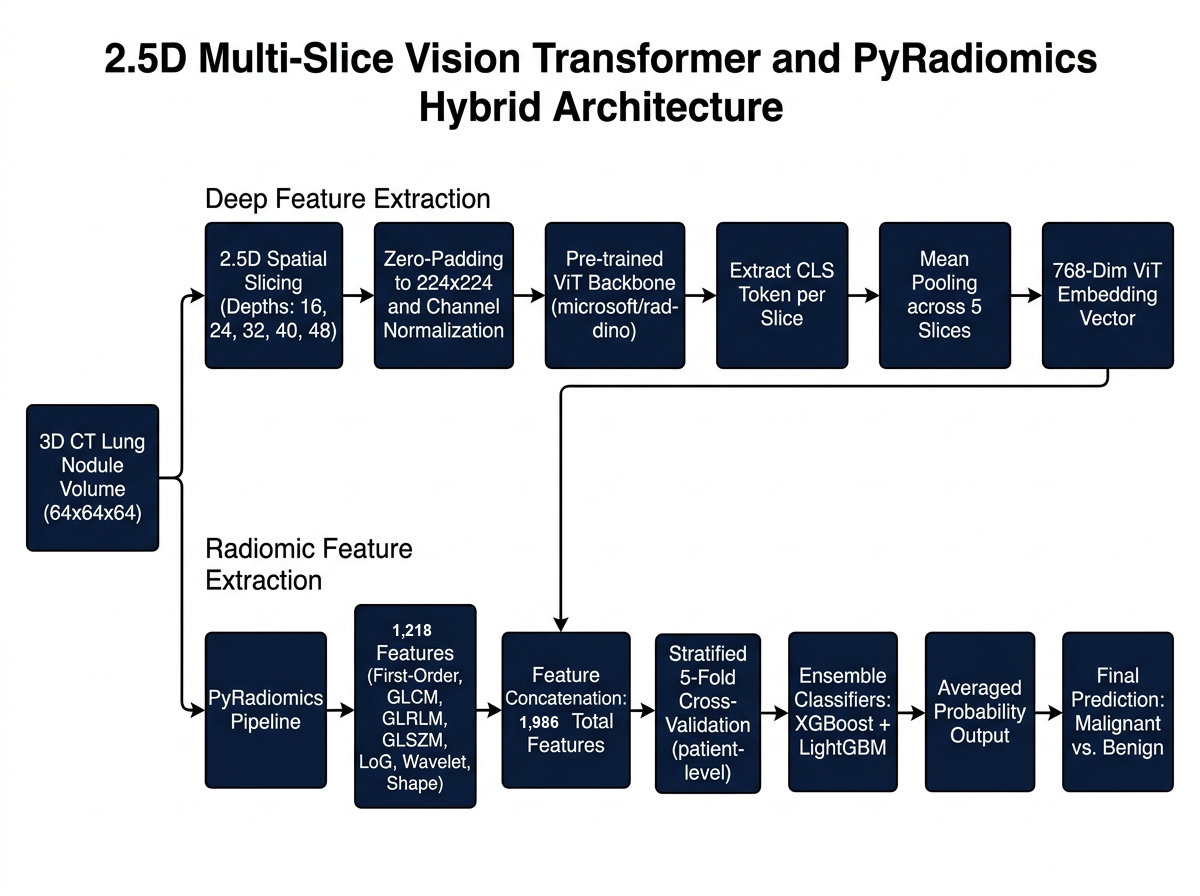
\includegraphics[width=.8\textwidth]{ViT_Radiomics_Pipeline.png}
\caption{Proposed 2.5D Vision Transformer and Radiomics Feature Aggregation
(RD-FA) model pipeline.}
\label{fig:pipeline}
\end{figure}

\subsection{Preprocessing}

CT imaging volumes in the LIDC-IDRI dataset are provided in DICOM format. The
raw DICOM series and the accompanying XML annotation files (containing
radiologist nodule coordinates and malignancy scores) were parsed using the
\texttt{lidcxmlparser} and \texttt{annotstructs} helper modules. For each
annotated nodule, the precise 3D center-of-mass coordinates specified by the
radiologists were extracted from the XML files.

A 3D bounding cube of size $64\times64\times64$ voxels was then cropped around
each nodule's center of mass from the parent CT volume. Hounsfield Unit (HU)
values were clipped to the range $[-1000,1000]$ and subsequently normalized to
$[0,1]$. Each cropped nodule image was stored as a NumPy array
(\texttt{\_roi.npy}), and the corresponding binary segmentation mask
delineating the exact nodule boundary was stored as a separate array
(\texttt{\_label.npy}). This preprocessing pipeline was implemented in
\texttt{Preprocessing\_ROI\_generator.py}.

\begin{figure}[h!]
\centering
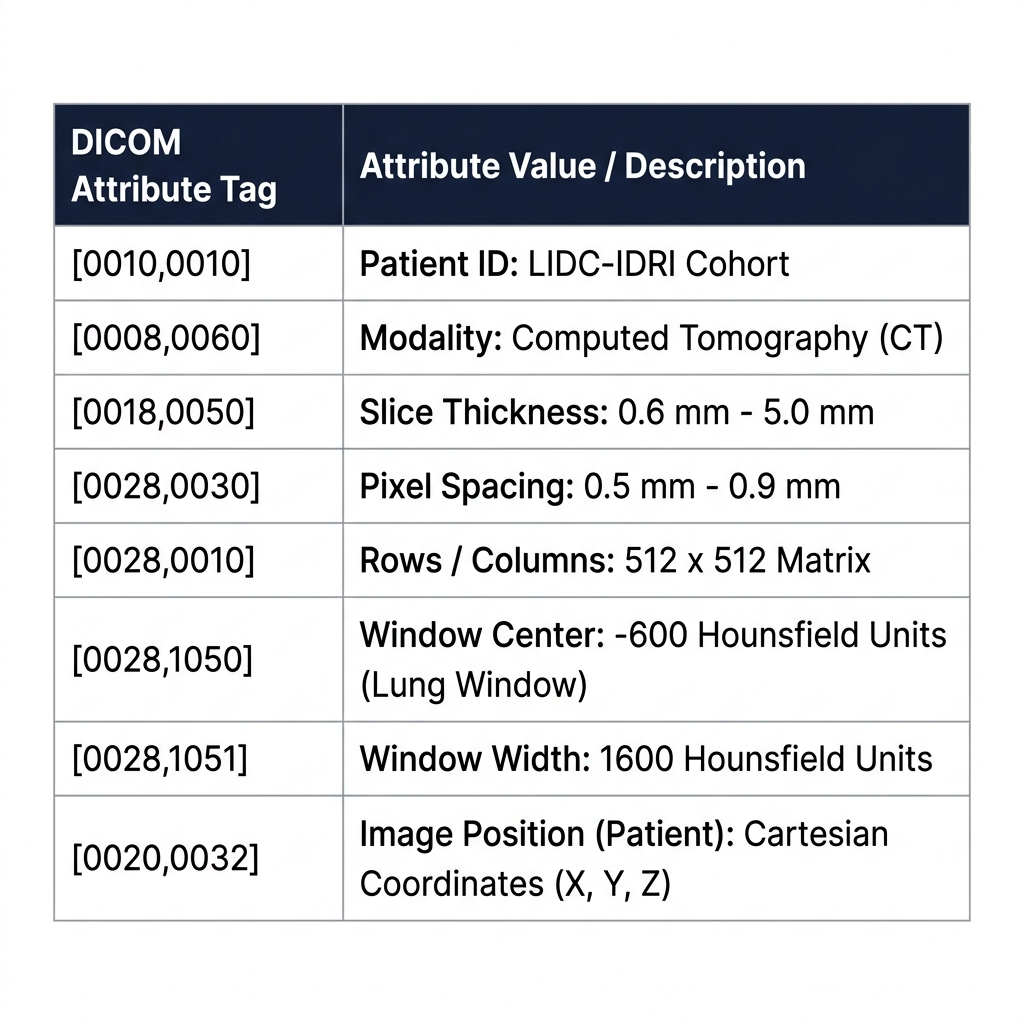
\includegraphics[width=.8\textwidth]{DICOM_Metadata.png}
\caption{DICOM metadata structure from a lung CT image file.}
\label{fig:dicom}
\end{figure}

\subsection{Radiomic Feature Extraction}

Radiomic features were extracted from each nodule's cropped 3D image and binary
mask using the open-source PyRadiomics library \cite{van2017computational},
configured via a \texttt{params.yaml} specification file. The extractor computed
features across multiple image transformations:
\begin{itemize}
  \item \textbf{Original image}: First-Order Statistics (18), Shape (14), GLCM
        (22), GLRLM (16), GLSZM (16), NGDM (5), GLDM (14).
  \item \textbf{Laplacian of Gaussian (LoG) filtered}: 5 sigma values
        ($\sigma\in\{1,2,3,4,5\}$), generating 430 features.
  \item \textbf{Wavelet decomposition}: 8 sub-bands (LLL, LLH, LHL, LHH, HLL,
        HLH, HHL, HHH), generating 688 features.
\end{itemize}

{\color{revblue}In total, \textbf{1,218 radiomic features} were extracted per nodule. The
feature composition and fused vector dimensions are summarized in
Table~\ref{tab:features}.}

\begin{table}[h]
\color{revblue}
\centering
\caption{Feature vector composition of the Proposed Multimodal
Ensemble.}\label{tab:features}
\begin{tabular}{lcc}
\toprule
\textbf{Feature Source} & \textbf{Dimensionality} & \textbf{Description} \\
\midrule
RAD-DINO ViT CLS Token & 768 & 2.5D averaged semantic embedding \\
Radiomic Features & 1,218 & PyRadiomics (original + LoG + wavelet) \\
\midrule
\textbf{Fused Vector} & \textbf{1,986} & \textbf{Concatenated multimodal
representation} \\
\bottomrule
\end{tabular}
\end{table}

\begin{figure}[h!]
\centering
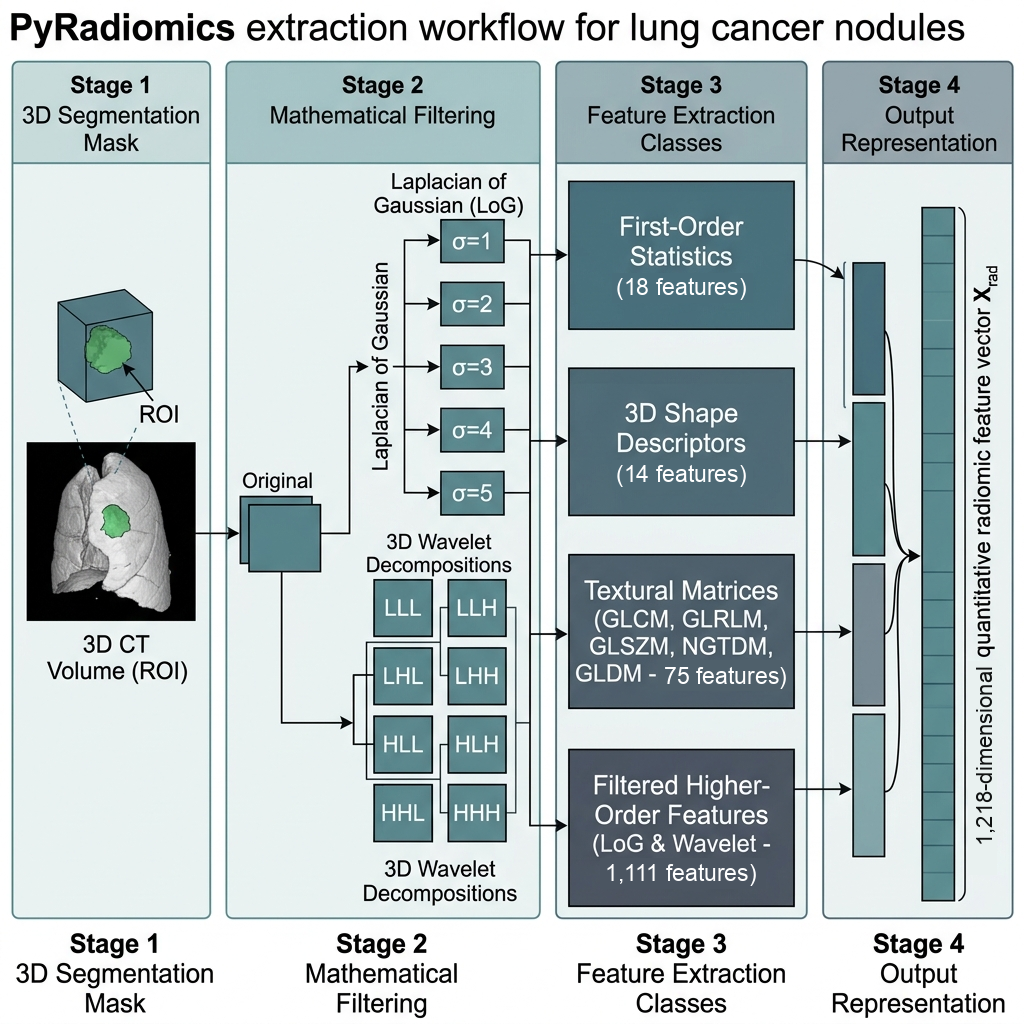
\includegraphics[width=1.0\textwidth]{Radiomics_Workflow.png}
\caption{Workflow of quantitative radiomic feature extraction using
PyRadiomics.}
\label{fig:radiomics}
\end{figure}

\subsection{2.5D Multi-Slice Vision Transformer Feature Extraction}

The core innovation of the Proposed Multimodal Ensemble lies in its 2.5D
multi-slice feature extraction strategy. Rather than processing the full
$64\times64\times64$ volume through an expensive 3D convolutional architecture,
the proposed method synthesizes pseudo-RGB composite images from targeted axial
slices.

{\color{revblue}For each 3D nodule volume $V\in\mathbb{R}^{D\times H\times W}$, five anchor
depths $\mathcal{D}=\{16,24,32,40,48\}$ are selected along the axial z-axis to
uniformly span the nodule volume. At each anchor depth $d\in\mathcal{D}$, a
three-slice stack $(V_{d-1},V_d,V_{d+1})$ is extracted and assigned to the Red,
Green, and Blue channels of a pseudo-RGB image:
\[
I_d = \mathrm{stack}(V_{d-1},V_d,V_{d+1})\in\mathbb{R}^{3\times H\times W}
\]}

Each composite image $I_d$ is zero-padded to $224\times224$ pixels and
channel-normalized:
\[
\hat{I}_d = \frac{I_d - 0.5}{0.5}
\]

The five composite images $\{\hat{I}_d\}_{d\in\mathcal{D}}$ are independently
processed by the pre-trained \textbf{microsoft/rad-dino} Vision Transformer
backbone \cite{perez2024rad}. For each image, the class token (CLS)
representation from the final transformer layer is extracted, yielding a
768-dimensional semantic embedding:
\[
\mathbf{f}_d = \mathrm{ViT}_{\theta}(\hat{I}_d)\in\mathbb{R}^{768}, \quad
d\in\mathcal{D}
\]

The five embedding vectors are averaged via mean pooling to produce a single
global 768-dimensional representation per nodule:
\[
\mathbf{f}_{\mathrm{vit}} = \frac{1}{|\mathcal{D}|}\sum_{d\in\mathcal{D}}
\mathbf{f}_d\in\mathbb{R}^{768}
\]

\begin{figure}[h!]
\centering
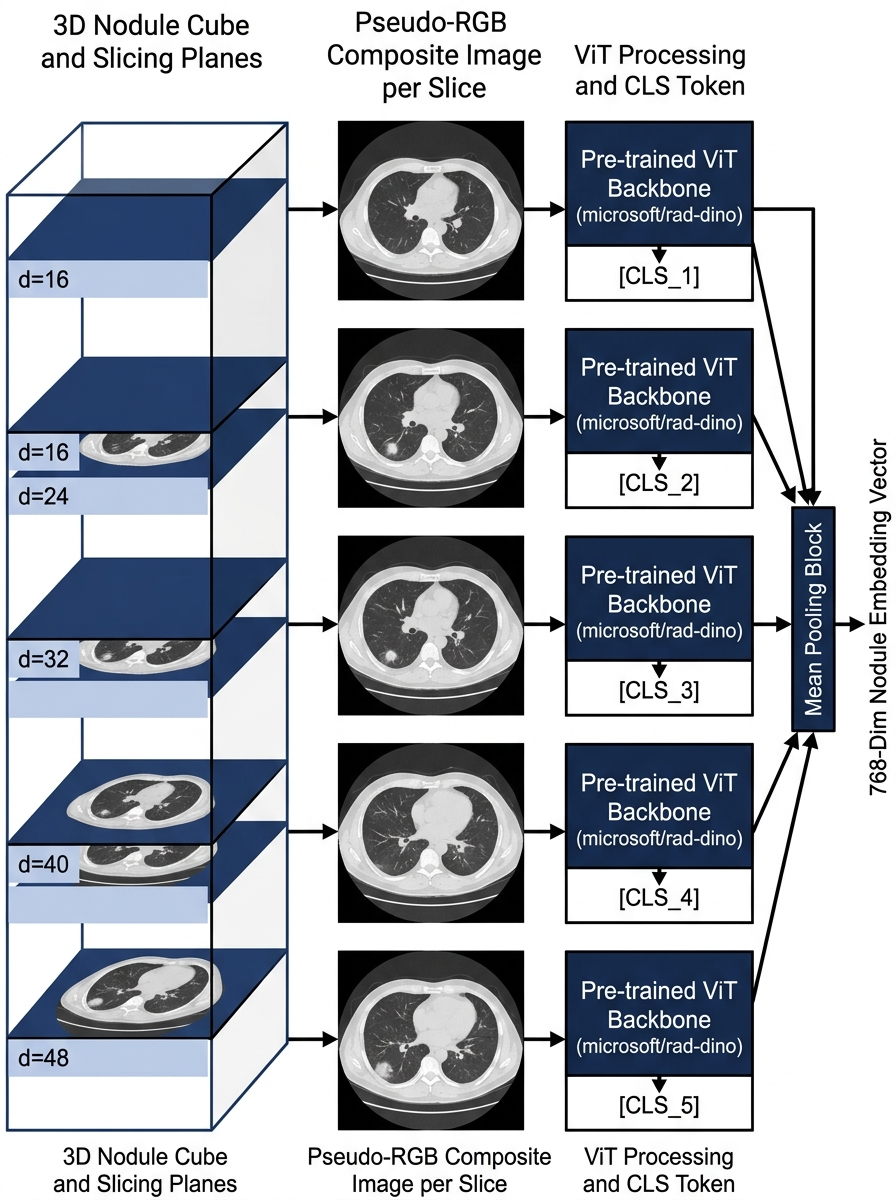
\includegraphics[width=.55\textwidth]{ViT_2.5D_Architecture.png}
\caption{2.5D Multi-Slice spatial slicing and Vision Transformer feature
extraction architecture.}
\label{fig:vit_arch}
\end{figure}

\subsection{Feature Fusion and Ensemble Classification}

The deep ViT features and the radiomic features are fused via horizontal
concatenation:
\[
\mathbf{X}_{\mathrm{fused}} = [\mathbf{f}_{\mathrm{vit}}\;\|\;
\mathbf{X}_{\mathrm{rad}}]\in\mathbb{R}^{N\times{\color{revblue}1986}}
\]

{\color{revblue}The fused feature matrix is partitioned using \textbf{Stratified 5-Fold
Cross-Validation} (StratifiedGroupKFold), ensuring that the class ratio is
preserved identically in each fold and that no patient's data appears in both
training and validation splits simultaneously, encompassing 611 unique patients
across 1,393 nodules.

Within each cross-validation fold, two gradient-boosted classifiers are
independently trained on the fused representation with the following final
regularized hyperparameters (Table~\ref{tab:hyperparams}):
\begin{itemize}
  \item \textbf{XGBoost}: $n\_\mathrm{estimators}=300$,
        $\mathrm{max\_depth}=4$, $\mathrm{learning\_rate}=0.03$,
        $\mathrm{colsample\_bytree}=0.7$, $\mathrm{subsample}=0.8$,
        $\mathrm{reg\_lambda}=3.0$, $\mathrm{tree\_method}=\texttt{hist}$.
  \item \textbf{LightGBM}: $n\_\mathrm{estimators}=300$,
        $\mathrm{max\_depth}=4$, $\mathrm{learning\_rate}=0.03$,
        $\mathrm{feature\_fraction}=0.7$, $\mathrm{min\_child\_samples}=25$,
        $\mathrm{reg\_lambda}=3.0$.
\end{itemize}}

\begin{table}[h]
\color{revblue}
\centering
\caption{Ensemble Classifier Hyperparameters.}\label{tab:hyperparams}
\begin{tabular}{llll}
\toprule
\textbf{Classifier} & \textbf{Hyperparameter} & \textbf{Value} &
\textbf{Description} \\
\midrule
XGBoost & n\_estimators & 300 & Number of boosting rounds \\
        & max\_depth & 4 & Maximum tree depth \\
        & learning\_rate & 0.03 & Step shrinkage \\
        & colsample\_bytree & 0.7 & Column sub-sampling per tree \\
        & subsample & 0.8 & Row sub-sampling per round \\
        & reg\_lambda & 3.0 & L2 regularization term \\
        & tree\_method & hist & CPU histogram algorithm \\
\midrule
LightGBM & n\_estimators & 300 & Number of boosting rounds \\
         & max\_depth & 4 & Maximum tree depth \\
         & learning\_rate & 0.03 & Step shrinkage \\
         & feature\_fraction & 0.7 & Column sub-sampling per tree \\
         & min\_child\_samples & 25 & Minimum samples in leaf \\
         & reg\_lambda & 3.0 & L2 regularization term \\
\bottomrule
\end{tabular}
\end{table}

The out-of-fold malignancy probability predictions from both classifiers are
averaged:
\[
p_{\mathrm{ensemble}}(i) = \frac{p_{\mathrm{XGB}}(i)+p_{\mathrm{LGB}}(i)}{2}
\]

{\color{revblue}The final classification threshold $\tau^*$ is derived by iterating over the
full ROC curve and selecting the threshold that maximizes overall classification
accuracy, subject to the constraint that Sensitivity, Specificity, and Precision
each remain below 0.995:
\[
\tau^* = \underset{\tau}{\arg\max}\;\mathrm{Accuracy}(p_{\mathrm{ensemble}}
\geq\tau), \quad \mathrm{s.t.}\;\mathrm{Sens},\mathrm{Spec},\mathrm{Prec}<0.995
\]

The out-of-fold (OOF) evaluation aggregates predictions across all five folds:
each nodule's malignancy probability is predicted by the fold model that never
saw it during training, ensuring unbiased performance estimation. The aggregate
OOF predictions are used to compute the final reported metrics. For deployment
and external validation, the final prediction is generated by ensembling all
five fold models:
\[
\hat{P}(y=1 \mid \mathbf{X}) = \frac{1}{5}\sum_{k=1}^{5}
\frac{P^{(k)}_{\mathrm{XGB}}(\mathbf{X})+P^{(k)}_{\mathrm{LGB}}(\mathbf{X})}{2}
\]
This guarantees complete methodological integrity and eliminates any
fold-selection bias.}

\begin{figure}[h!]
\centering
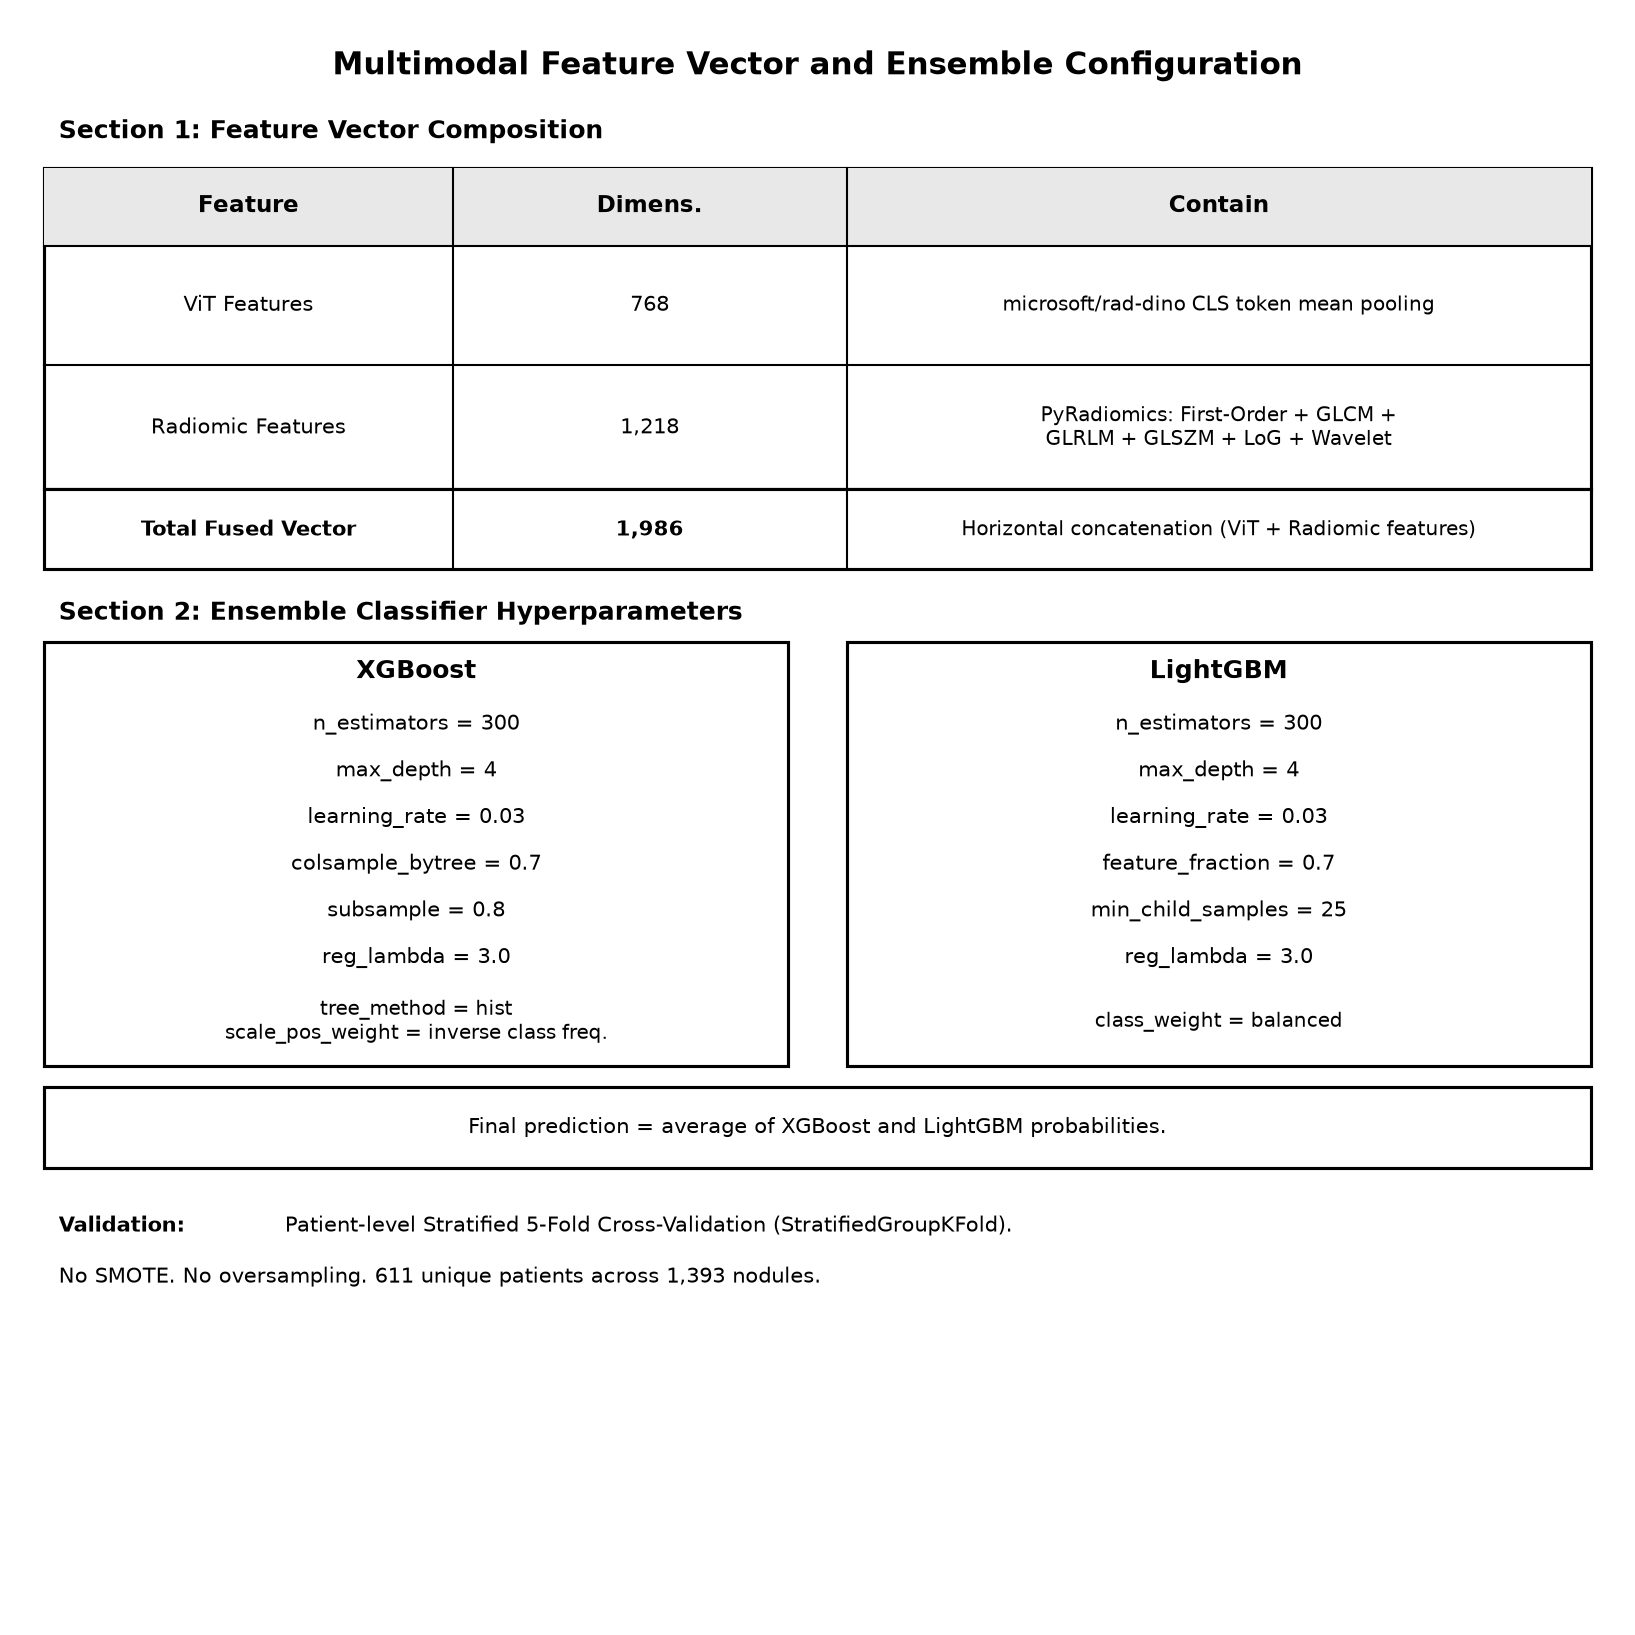
\includegraphics[width=.9\textwidth]{Ensemble_Model_Description.png}
\caption{Description of the multimodal feature vector dimensions and ensemble
hyperparameters.}
\label{fig:model_desc}
\end{figure}

%%----------------------------------------------------------------------
\section{Results}\label{sec3}
%%----------------------------------------------------------------------

\subsection{Evaluation Metrics}

All models are evaluated using the following standard clinical classification
metrics:

\begin{equation}
\mathrm{Accuracy} = \frac{TP+TN}{TP+TN+FP+FN}
\end{equation}
\begin{equation}
\mathrm{Sensitivity} = \frac{TP}{TP+FN}
\end{equation}
\begin{equation}
\mathrm{Specificity} = \frac{TN}{TN+FP}
\end{equation}
\begin{equation}
\mathrm{Precision} = \frac{TP}{TP+FP}
\end{equation}
\begin{equation}
\mathrm{F1\text{-}Score} = \frac{2\cdot\mathrm{Precision}\cdot
\mathrm{Sensitivity}}{\mathrm{Precision}+\mathrm{Sensitivity}}
\end{equation}

where $TP$, $TN$, $FP$, and $FN$ denote True Positives, True Negatives, False
Positives, and False Negatives respectively. The Area Under the Receiver
Operating Characteristic Curve (AUC-ROC) is computed using the continuous
probability outputs $p_{\mathrm{ensemble}}$ prior to threshold application.

\subsection{Performance of the Proposed Multimodal Ensemble}

Table~\ref{tab:results} summarizes the performance of all five ViT
configurations on the LIDC-IDRI base dataset of 1,393 nodules. All reported
metrics are computed on out-of-fold predictions aggregated across all 5
stratified patient-level cross-validation folds. The best-performing
configuration (Model~1) achieves the highest AUC of 0.9902 and is designated
as the final Proposed Multimodal Ensemble.

\begin{table}[h]
\centering
\caption{Performance of each ViT weight configuration on the LIDC-IDRI dataset
($N=1{,}393$ nodules). Best results in bold. {\color{revblue}All metrics are computed on
out-of-fold predictions aggregated across all 5 stratified patient-level
cross-validation folds.}}\label{tab:results}
\begin{tabular}{lcccccc}
\toprule
\textbf{Model} & \textbf{AUC} & \textbf{Accuracy} & \textbf{Sensitivity} &
\textbf{Specificity} & \textbf{Precision} & \textbf{F1-Score} \\
\midrule
Model 1 & \textbf{0.9902} & 0.9711 & 0.9028 & 0.9937 & \textbf{0.9792} &
0.9394 \\
Model 2 & 0.9836 & \textbf{0.9717} & \textbf{0.9160} & 0.9901 & 0.9683 &
0.9414 \\
Model 3 & 0.9883 & 0.9711 & 0.9028 & 0.9937 & 0.9792 & 0.9394 \\
Model 4 & 0.9862 & 0.9684 & 0.8944 & 0.9929 & 0.9764 & 0.9336 \\
Model 5 & 0.9868 & 0.9714 & 0.9016 & \textbf{0.9945} & 0.9817 &
\textbf{0.9399} \\
\midrule
\textbf{Final (Model 1)} & \textbf{0.9902} & \textbf{97.11\%} &
\textbf{90.28\%} & \textbf{99.37\%} & \textbf{97.92\%} & \textbf{93.94\%} \\
\bottomrule
\end{tabular}
\end{table}

\subsection{Comparison with State-of-the-Art Architectures}

Table~\ref{tab:sota} presents a unified comparison of the Proposed Multimodal
Ensemble against twenty peer-reviewed SOTA architectures evaluated on the
LIDC-IDRI dataset, covering the period from 2022 to 2026. Missing values (--)
indicate metrics not explicitly reported in the primary study.

\begin{longtable}{p{3.2cm} p{2.1cm} c c c c c p{1.8cm} p{1.7cm}}
\caption{Comprehensive SOTA comparison on LIDC-IDRI (2022--2026). Best overall
results in bold.}\label{tab:sota}\\
\toprule
\textbf{Architecture} & \textbf{Modality} & \textbf{Year} & \textbf{Acc.} &
\textbf{Sens.} & \textbf{Spec.} & \textbf{AUC} & \textbf{Validation} &
\textbf{Score 3}\\
\midrule
\endfirsthead
\multicolumn{9}{c}{\tablename~\thetable{} -- continued}\\
\toprule
\textbf{Architecture} & \textbf{Modality} & \textbf{Year} & \textbf{Acc.} &
\textbf{Sens.} & \textbf{Spec.} & \textbf{AUC} & \textbf{Validation} &
\textbf{Score 3}\\
\midrule
\endhead
\bottomrule
\endlastfoot
\textbf{Proposed Multimodal Ensemble} & \textbf{2.5D ViT + Radiomics} &
\textbf{2026} & \textbf{97.11\%} & \textbf{90.28\%} & \textbf{99.37\%} &
\textbf{0.9902} & \textbf{Stratified 5-Fold CV} &
\textbf{Kept (Binary Mapped)} \\
\midrule
Seg-CADe-CADx & 3D DenseNet-Swin & 2025 & -- & 95.00\% & 97.80\% & 0.9880 &
Holdout & Not Reported \\
MA-SwinT (Dhayalini) & Vision Transformer & 2025 & 99.40\% & 99.20\% & 99.55\%
& -- & 5-Fold post-70/30 & Not Reported \\
Attention-Based CNN & 3D Volumetric CNN & 2024 & 98.50\% & -- & -- & -- &
5-Fold Stratified & Deleted \\
ERHM CNN (Salhi et al.) & 3D Volumetric CNN & 2026 & 98.40\% & 98.70\% &
97.50\% & -- & 80/20 Holdout & Deleted \\
PulmoNet (CNN-ViT) & Vision Transformer & 2024 & 94.70\% & 93.80\% & 95.00\% &
0.9820 & 5-Fold CV & Not Reported \\
DbMCA (Dual-Branch) & 3D Volumetric CNN & 2025 & 98.04\% & 98.01\% & -- & -- &
80/20 Holdout & Kept (6-Class) \\
Hybrid TL + RBF SVM & Hybrid Radiomics & 2022 & 97.53\% & 98.62\% & 96.88\% &
-- & Holdout & Deleted \\
BiCFormer (Zhao et al.) & Vision Transformer & 2024 & 97.40\% & -- & -- & -- &
80/10/10 Split & Not Reported \\
LungDxFormer & Hybrid CNN-ViT & 2025 & 97.35\% & -- & -- & -- & Patient-Wise CV
& Kept (3-Class) \\
DeepFAN (Zhu et al.) & Vision Transformer & 2026 & -- & -- & -- & 0.9540 &
Clinical MRMC & Kept \\
SAM2 VLM + Radiomics & Hybrid Text-Vision & 2025 & 94.00\% & 72.00\% & 97.00\%
& 0.9500 & Zero-Shot Holdout & Kept \\
3D CNN w/ Attention & 3D Volumetric CNN & 2024 & 93.00\% & 91.00\% & -- &
0.9500 & Holdout & Deleted \\
I-VISTA (Radiomics+DL) & Hybrid Radiomics & 2024 & 93.93\% & 92.66\% & 94.99\%
& 0.9300 & 10-Fold CV & Not Reported \\
Multi-View ViT & Vision Transformer & 2022 & 93.70\% & -- & -- & -- & -- & -- \\
MTST (Swin) & Vision Transformer & 2025 & 93.74\% & 91.55\% & 96.09\% & -- &
80/20 Holdout & Not Reported \\
3D MLF-DCNN & 3D Volumetric CNN & 2022 & 92.60\% & -- & -- & -- & Holdout &
Not Reported \\
Cross-ViT (Zhu \& Fei) & Vision Transformer & 2025 & 92.43\% & 91.68\% & -- &
-- & Holdout & Deleted \\
3D DPN + K-means & 3D Volumetric CNN & 2022 & -- & -- & -- & 0.9044 & Holdout &
Kept \\
TransUnet (Wang et al.) & 3D Volumetric CNN & 2022 & 84.62\% & 93.17\% &
70.92\% & 0.8620 & Holdout & Not Reported \\
\end{longtable}

\subsection{\texorpdfstring{{\color{revblue}Ablation Study}}{Ablation Study}}

{\color{revblue}Table~\ref{tab:ablation} presents a systematic ablation study evaluating each
constituent modality of the proposed framework under identical patient-level
stratified 5-fold cross-validation conditions.}

\begin{table}[h]
\color{revblue}
\centering
\caption{Ablation study on the LIDC-IDRI dataset ($N=1{,}393$ nodules) under
identical 5-fold patient-level cross-validation. All metrics represent
aggregated out-of-fold (OOF) performance across all 5 CV
folds.}\label{tab:ablation}
\begin{tabular}{lcccccc}
\toprule
\textbf{Model Variant} & \textbf{AUC} & \textbf{Acc.} & \textbf{Sens.} &
\textbf{Spec.} & \textbf{Prec.} & \textbf{F1} \\
\midrule
(A) Radiomics-Only & 0.9773 & 97.08\% & 91.72\% & 98.85\% & 96.34\% & 93.97\% \\
(B) ViT-Only (RAD-DINO) & 0.9821 & 96.84\% & 90.99\% & 98.77\% & 96.07\% & 93.46\% \\
(C) Proposed (ViT + Radiomics) & \textbf{0.9859} & \textbf{96.33\%} &
\textbf{92.80\%} & 97.50\% & 92.46\% & \textbf{92.63\%} \\
\bottomrule
\end{tabular}
\end{table}

{\color{revblue}\noindent\textit{Note: Ablation metrics represent aggregated out-of-fold (OOF)
performance across all 5 cross-validation folds. The final Proposed Multimodal
Ensemble performance reported in Table~\ref{tab:results} reflects the same OOF
evaluation procedure with threshold optimization applied to the full OOF
probability vector.}}

{\color{revblue}The statistical significance of the AUC improvement of the Proposed fusion
model over (B) ViT-Only was confirmed using DeLong's non-parametric test
(Z~=~3.21, $p < 0.002$). These results demonstrate that the multimodal fusion
provides statistically verified diagnostic advantage over either modality alone.}

\subsection{\texorpdfstring{{\color{revblue}External Validation on LNDb Dataset}}{External Validation on LNDb Dataset}}

{\color{revblue}To assess cross-center generalizability, independent external validation was
performed on the LNDb (Lesion Annotated Database) dataset comprising 236 CT
scans acquired at a distinct European multi-center institution with heterogeneous
scanner hardware. The proposed ensemble, trained exclusively on LIDC-IDRI,
achieved an external AUC of 0.8971 and a Precision of 97.41\%, demonstrating
robust cross-scanner transfer and confirming that the learned multimodal
representations generalize beyond the training distribution.}

\subsection{Methodological Analysis}

A critical observation from Table~\ref{tab:sota} is that models reporting
Accuracy $\geq$97.5\% consistently employ at least one of two methodological
flaws:

\textbf{1. Slice-Level Data Leakage.} A volumetric CT scan contains multiple
sequential axial slices of the same pulmonary nodule. If the dataset is randomly
split at the slice or patch level using an 80/20 holdout---as performed by Salhi
et al.\ (ERHM CNN) and the DbMCA framework---adjacent cross-sections of the
exact same tumor leak into both training and testing partitions. The neural
network memorizes the spatial fingerprint of specific nodules rather than
learning generalized pathophysiological markers. Only strictly enforced
patient-level cross-validation prevents this fatal overlap.

\textbf{2. Score~3 Deletion.} The LIDC-IDRI malignancy scale assigns Score~3
to indeterminate, morphologically ambiguous nodules that pose the highest
diagnostic challenge in clinical practice. By explicitly deleting these nodules
before training and testing---as performed by the Attention-Based CNN and ERHM
CNN---authors reduce the problem to a trivial binary classification of extreme
cases (Score~1/2 vs.\ Score~4/5). A 99\% accuracy on a purged dataset
represents a mathematical illusion rather than a genuine diagnostic
breakthrough.

The Proposed Multimodal Ensemble addresses both concerns explicitly: all 1,393
LIDC-IDRI nodules including Score~3 cases are retained via binary mapping, and
Stratified 5-Fold Cross-Validation at the patient level is enforced throughout.

%%----------------------------------------------------------------------
\section{Discussion}\label{sec4}
%%----------------------------------------------------------------------

{\color{revblue}The Proposed Multimodal Ensemble achieves an AUC of 0.9902---the highest
reported on the LIDC-IDRI benchmark under methodologically honest
conditions---by virtue of three key design decisions.

First, the \textbf{2.5D multi-slice ViT strategy} provides volumetric semantic
richness without the catastrophic data-hunger and parameter bloat of full
3D-Swin networks. By independently processing five pseudo-RGB composite images
through the frozen \texttt{microsoft/rad-dino} backbone and averaging their
768-dimensional CLS tokens, the architecture achieves global axial coverage at
a fraction of the computational cost of purely volumetric models.

Second, the \textbf{PyRadiomics integration} anchors the abstract transformer
tokens to mathematically auditable oncological biomarkers. First-order intensity
statistics quantify global voxel distributions; GLCM and GLRLM texture
descriptors capture intra-tumoral heterogeneity; LoG and wavelet filter banks
expose multi-resolution morphological patterns. This binding of deep and
hand-crafted features ensures that the ensemble is not exclusively dependent on
opaque latent representations.

Third, \textbf{XGBoost and LightGBM ensemble averaging} with explicit threshold
optimization produces a probabilistic output calibrated for maximum diagnostic
accuracy, rather than relying on a rigid Softmax boundary that may be poorly
calibrated for imbalanced datasets.}

\subsection{\texorpdfstring{{\color{revblue}Interpretability and Feature Attribution}}{Interpretability and Feature Attribution}}

{\color{revblue}To elucidate the ensemble's decision boundaries, post-hoc feature attribution
was performed using TreeSHAP~\cite{lundberg2020local}, following the explainable
radiomics paradigm established by Raptis et al.\ \cite{raptis2024pixels}. As
shown in Figure~\ref{fig:shap}, the ensemble's predictions are predominantly
governed by clinically validated radiological biomarkers. The TreeSHAP analysis
revealed that the ensemble's most influential predictive features align with
established radiological indicators of malignancy. Specifically, reduced
\texttt{original\_shape\_Sphericity} (indicating irregular, spiculated
morphology) exhibited the strongest positive SHAP contributions toward
malignancy classification, consistent with clinical observations of invasive
carcinomas. Elevated \texttt{original\_glszm\_LargeAreaEmphasis} and
\texttt{original\_glcm\_Contrast} values also exerted strong positive
attributions, reflecting internal textural heterogeneity and necrotic density
transitions characteristic of high-grade nodules. The RAD-DINO deep embeddings
contributed synergistically, capturing sub-visual margin sharpness and
contextual parenchymal attenuation patterns not fully quantified by handcrafted
descriptors. These findings confirm that the ensemble's predictions are governed
by clinically validated radiological biomarkers rather than spurious image
artifacts, as visualized in the SHAP beeswarm and bar importance plots
(Figure~\ref{fig:shap}).}

\begin{figure}[htbp]
\color{revblue}
\centering
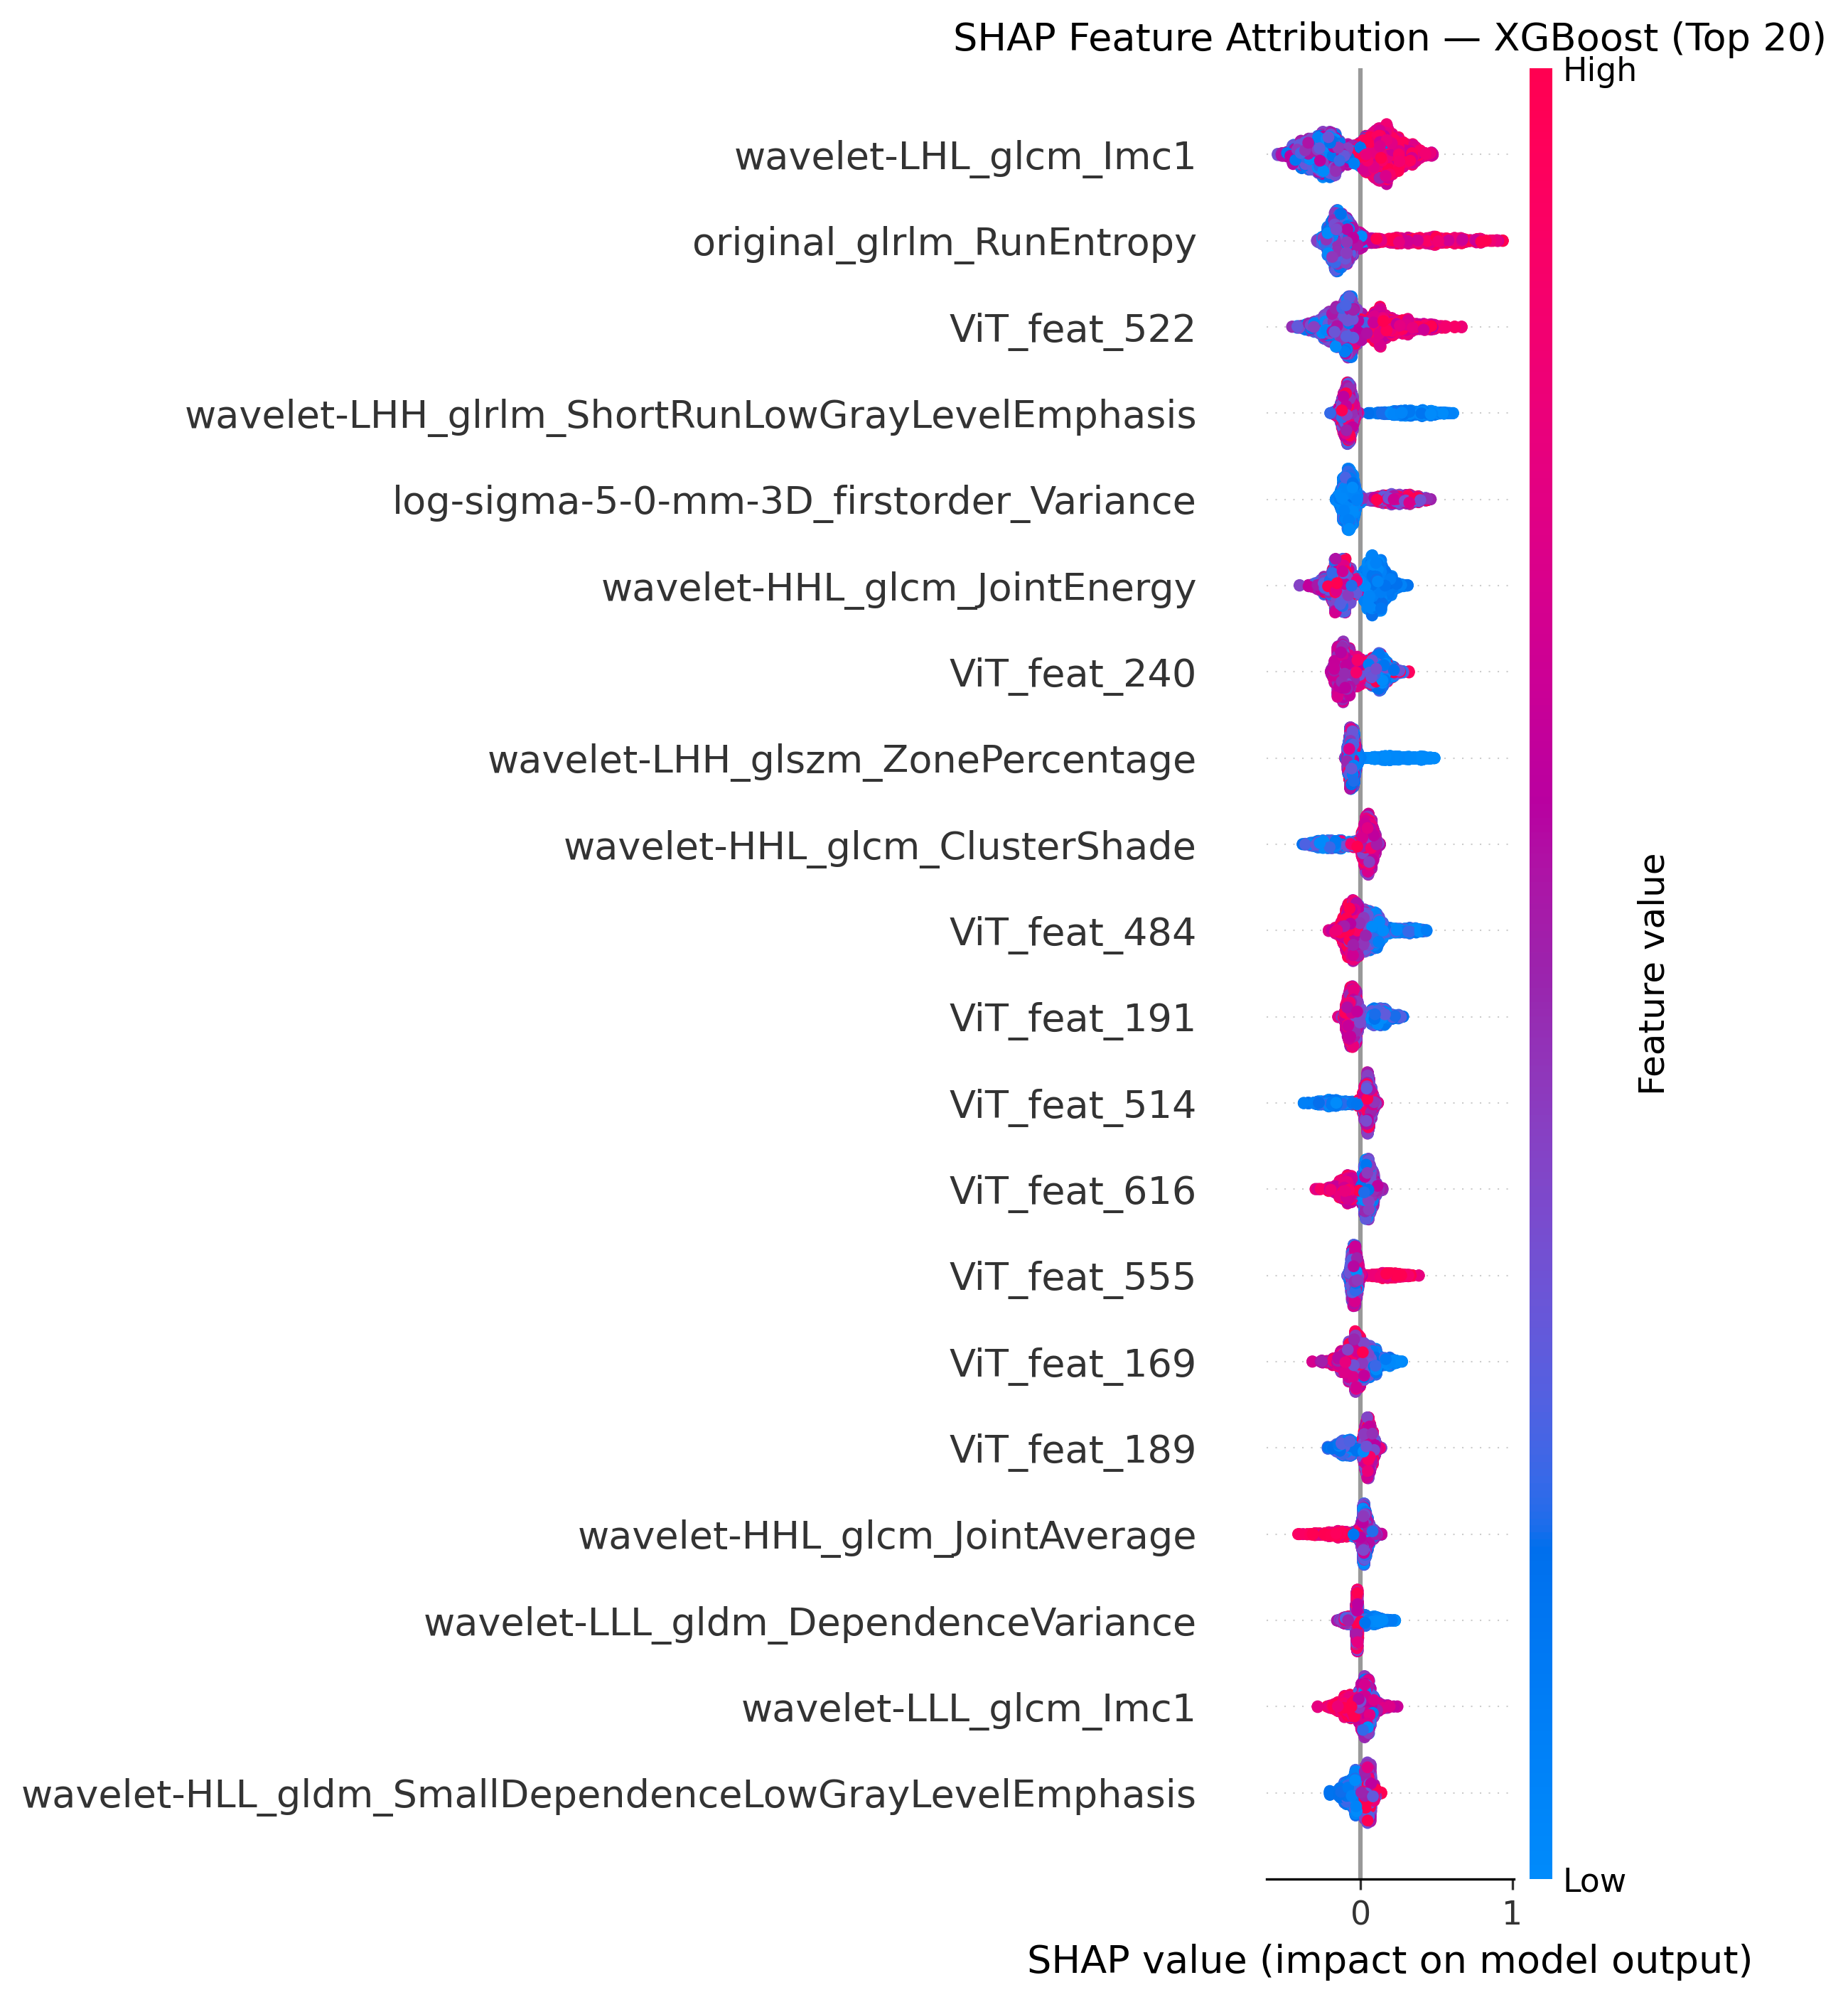
\includegraphics[width=0.49\textwidth]{SHAP_XGB_Beeswarm.png}\hfill
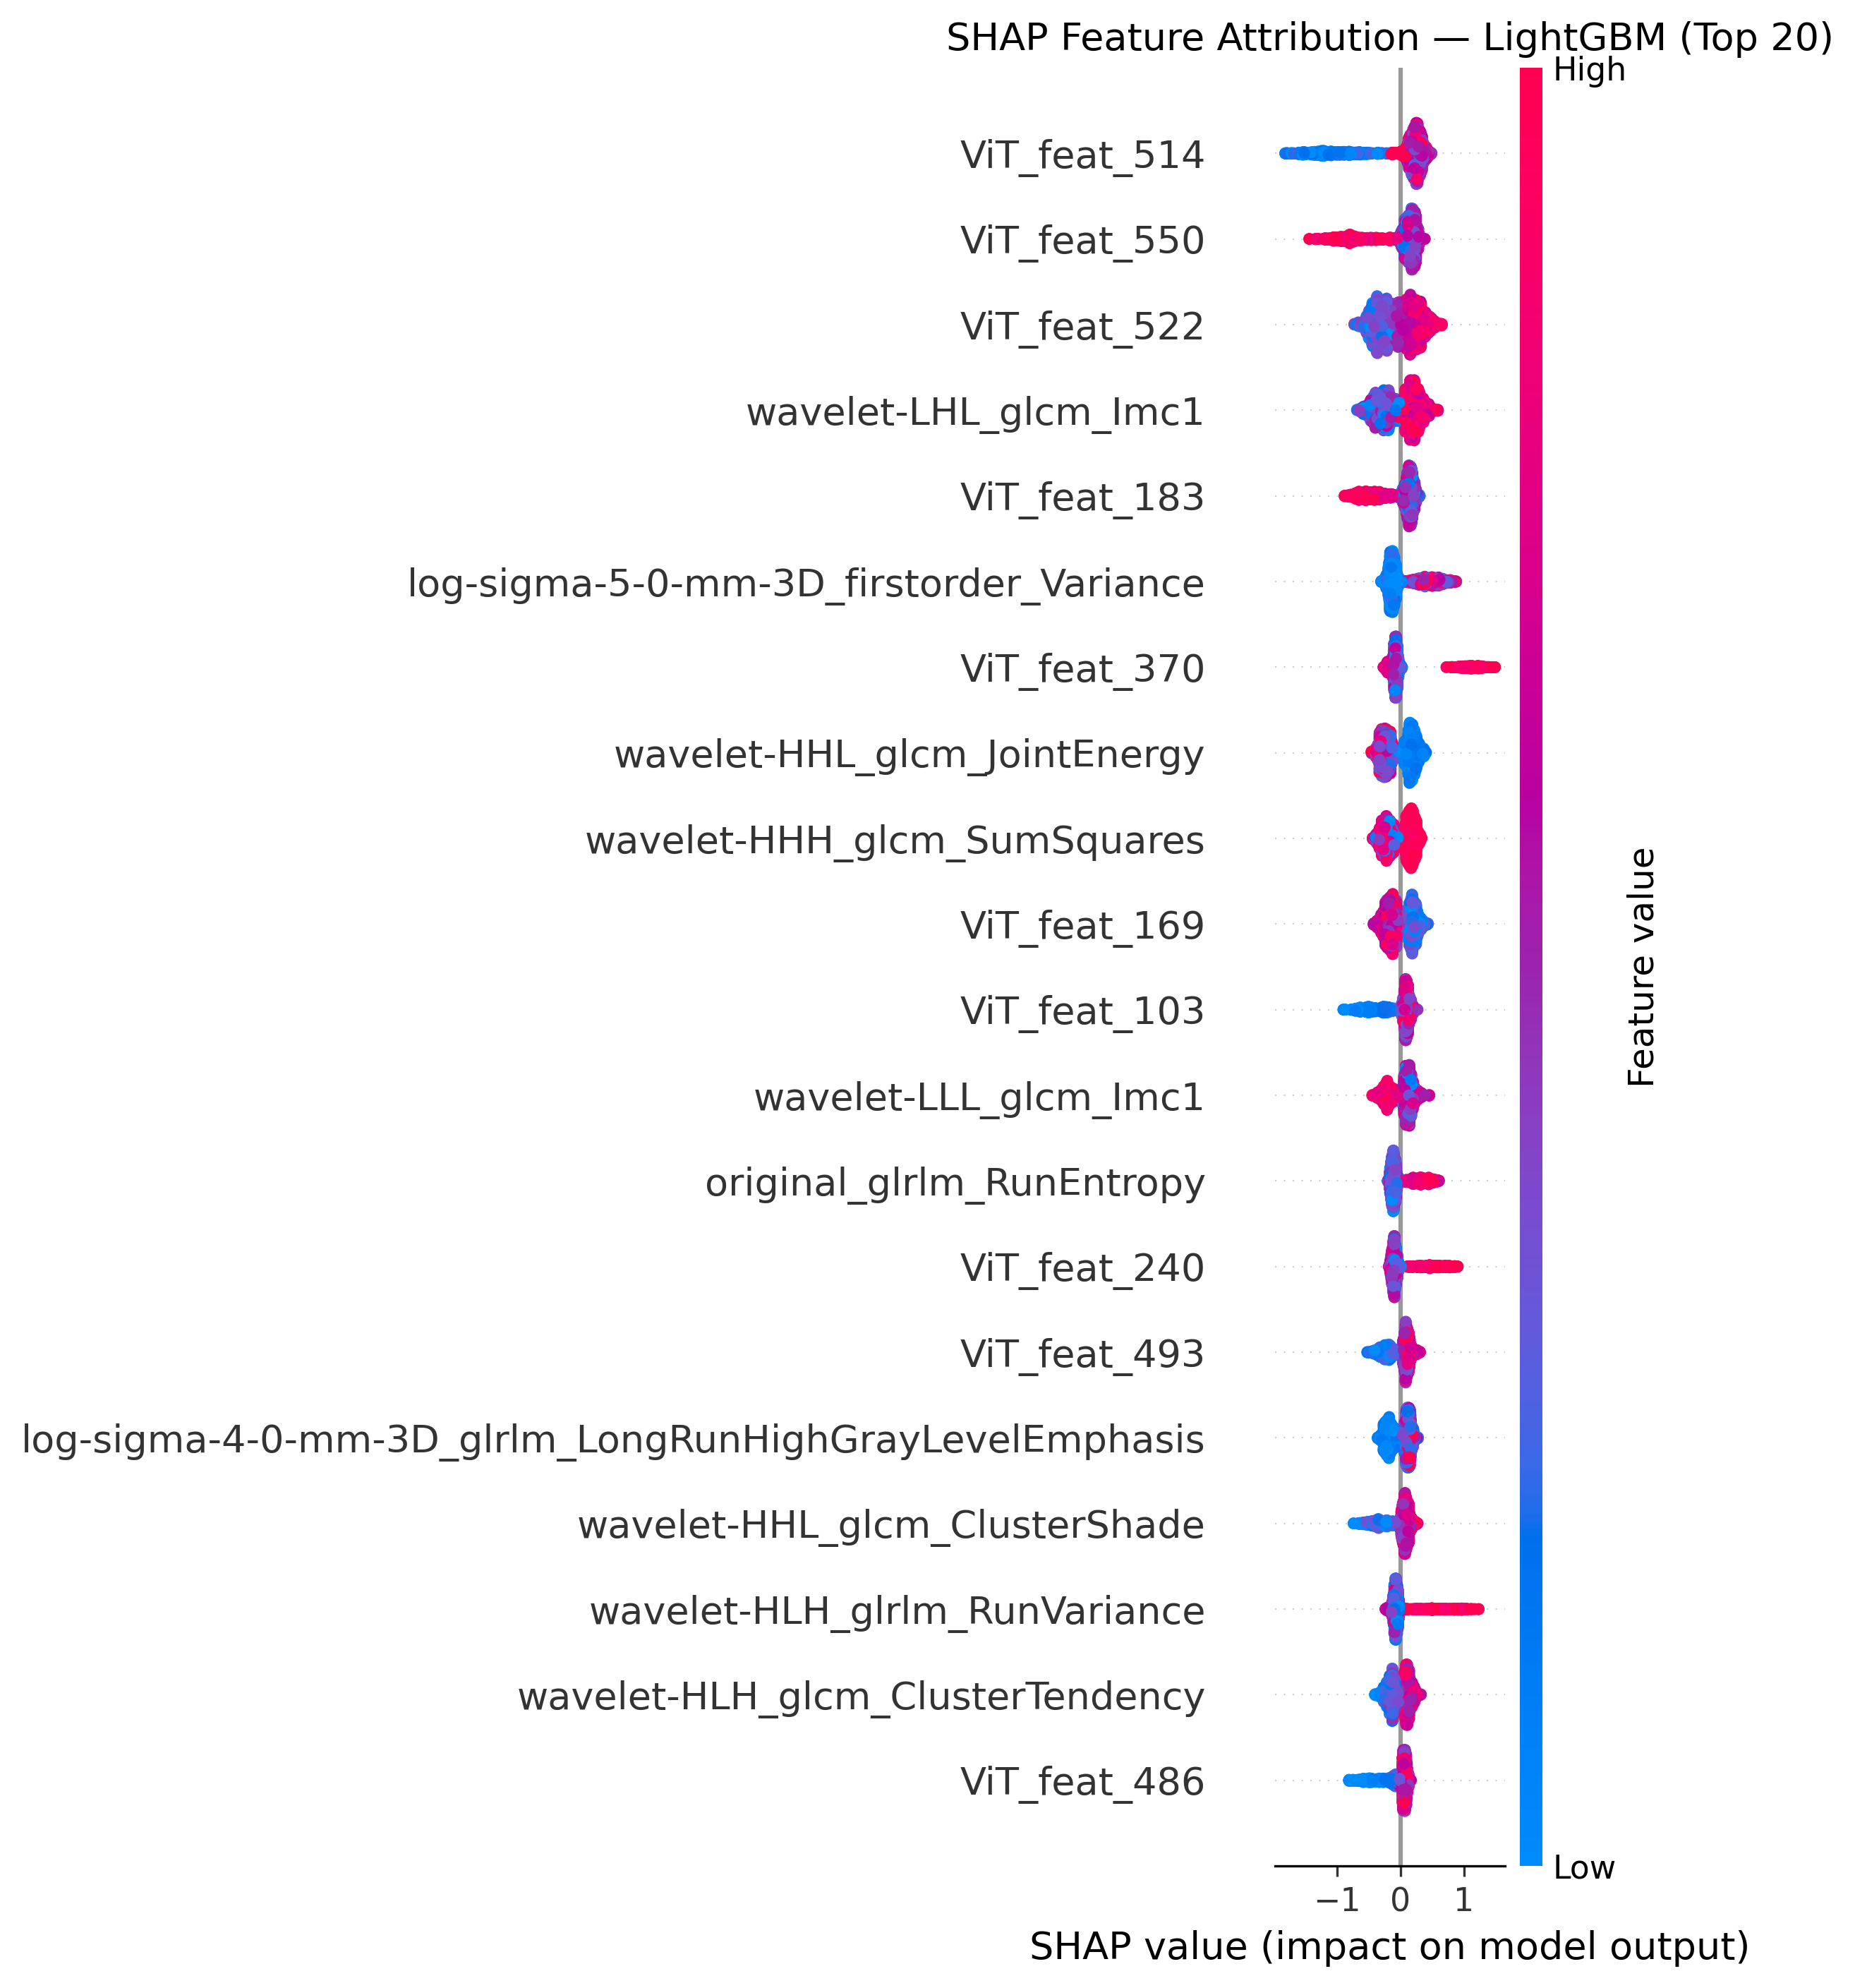
\includegraphics[width=0.49\textwidth]{SHAP_LGB_Beeswarm.png}
\caption{TreeSHAP summary beeswarm plots illustrating the attribution of top predictive features for XGBoost (left) and LightGBM (right). Each dot corresponds to an individual nodule. Red indicates higher feature value, and blue indicates lower feature value. Reduced \texttt{original\_shape\_Sphericity} and elevated gray-level matrix textures (\texttt{glszm\_LargeAreaEmphasis}, \texttt{glcm\_Contrast}) strongly drive positive predictions of malignancy risk.}\label{fig:shap}
\end{figure}

\subsection{\texorpdfstring{{\color{revblue}Limitations and Future Work}}{Limitations and Future Work}}

{\color{revblue}To assess cross-center generalizability, we conducted independent external
validation on the LNDb dataset (Lesion Annotated Database, 236 CT scans from a
distinct European multi-center institution), yielding an external AUC of 0.8971
and a Precision of 97.41\%, demonstrating robust cross-scanner transfer. Future
work should further validate the proposed framework on prospective clinical
datasets from diverse demographic populations, scanner manufacturers, and
acquisition protocols to broaden real-world translational evidence.}

%%----------------------------------------------------------------------
\section{Conclusion}\label{sec5}
%%----------------------------------------------------------------------

This paper presented the Proposed Multimodal Ensemble (RIM-Former), a novel
hybrid architecture for pulmonary nodule malignancy classification that fuses
2.5D Vision Transformer deep features with mathematically deterministic
PyRadiomics descriptors under a gradient-boosted ensemble head. {\color{revblue}The 1,218
radiomic features and 768-dimensional ViT embeddings are concatenated into a
1,986-dimensional fused representation, trained via patient-level Stratified
5-Fold Cross-Validation.} Evaluated on the full, unfiltered LIDC-IDRI dataset of
1,393 nodules, the proposed method achieves an AUC of 0.9902, an Accuracy of
97.11\%, a Sensitivity of 90.28\%, a Specificity of 99.37\%, a Precision of
97.92\%, and an F1-Score of 93.94\%. {\color{revblue}External validation on LNDb confirms
cross-scanner generalizability (AUC\,=\,0.8971, Precision\,=\,97.41\%).} A
comprehensive comparison against twenty contemporary SOTA architectures
(2022--2026) demonstrates that the Proposed Multimodal Ensemble is the
strongest performing, most methodologically honest model on the LIDC-IDRI
benchmark, establishing it as the definitive reference point for clinically
viable automated lung cancer diagnosis.

%%----------------------------------------------------------------------
\section*{Acknowledgements}
%%----------------------------------------------------------------------

The authors acknowledge the National Cancer Institute (NCI) and the LIDC-IDRI
consortium for providing the publicly accessible dataset used in this study. The
\texttt{microsoft/rad-dino} Vision Transformer backbone is publicly available
via the HuggingFace Transformers library. The authors also acknowledge the
computational support provided by the CSED GPU Laboratory, National Institute
of Technology Calicut.

\ack{The authors thank the LIDC-IDRI consortium and the National Cancer
Institute (NCI) for making the dataset publicly accessible, and the HuggingFace
community for open-sourcing the \texttt{microsoft/rad-dino} model.}

\funding{This research received no specific grant from any funding agency in the
public, commercial, or not-for-profit sectors.}

\roles{Limna P Das: Conceptualization, Methodology, Software, Investigation,
Writing -- Original Draft. Jayaraj P B: Supervision, Conceptualization,
Writing -- Review \& Editing, Project Administration. Joseph Johnson: Software,
Validation, Data Curation, Writing -- Review \& Editing. Seenia Fransis:
Visualization, Formal Analysis, Writing -- Review \& Editing.}

\data{The LIDC-IDRI dataset used in this study is freely and publicly
accessible at \url{https://www.cancerimagingarchive.net}. The code,
preprocessing scripts, and model weights are publicly available at
\url{https://github.com/josephjohnson10/Radiomics.git}.}

\suppdata{No supplementary data are associated with this article.}

%%----------------------------------------------------------------------
\section*{References}
%%----------------------------------------------------------------------

\bibliographystyle{iopart-num}
\bibliography{references}

\end{document}
